\documentclass[12pt]{article}

\usepackage{amssymb}
\usepackage{amsmath}
\usepackage{amsthm}
\usepackage{fullpage}
\usepackage{adjustbox}

\usepackage{tikz-cd}
\usetikzlibrary{calc,matrix,arrows}
\usetikzlibrary{decorations.pathmorphing}
\tikzset{curve/.style={settings={#1},to path={(\tikztostart)
    .. controls ($(\tikztostart)!\pv{pos}!(\tikztotarget)!\pv{height}!270:(\tikztotarget)$)
    and ($(\tikztostart)!1-\pv{pos}!(\tikztotarget)!\pv{height}!270:(\tikztotarget)$)
    .. (\tikztotarget)\tikztonodes}},
    settings/.code={\tikzset{quiver/.cd,#1}
        \def\pv##1{\pgfkeysvalueof{/tikz/quiver/##1}}},
    quiver/.cd,pos/.initial=0.35,height/.initial=0}

% TikZ arrowhead/tail styles.
\tikzset{tail reversed/.code={\pgfsetarrowsstart{tikzcd to}}}
\tikzset{2tail/.code={\pgfsetarrowsstart{Implies[reversed]}}}
\tikzset{2tail reversed/.code={\pgfsetarrowsstart{Implies}}}
% TikZ arrow styles.
\tikzset{no body/.style={/tikz/dash pattern=on 0 off 1mm}}

\usepackage{listings}

\definecolor{mygreen}{rgb}{0,0.6,0}
\definecolor{mygray}{rgb}{0.5,0.5,0.5}
\definecolor{mymauve}{rgb}{0.58,0,0.82}

\lstset{ %
  backgroundcolor=\color{white},   % choose the background color
  basicstyle=\footnotesize,        % size of fonts used for the code
  breaklines=true,                 % automatic line breaking only at whitespace
  captionpos=b,                    % sets the caption-position to bottom
  commentstyle=\color{mygreen},    % comment style
  escapeinside={\%*}{*)},          % if you want to add LaTeX within your code
  keywordstyle=\color{blue},       % keyword style
  stringstyle=\color{mymauve},     % string literal style
}

\usepackage{hyperref}
\hypersetup{colorlinks,citecolor=black,filecolor=black,linkcolor=black,urlcolor=black}
\usepackage{theoremref}

\newtheorem{thm}{Theorem}[section]
\newtheorem{cor}{Corollary}[thm]
\newtheorem{lem}[thm]{Lemma}
\newtheorem*{thm*}{Theorem}
\newtheorem*{cor*}{Corollary}
\newtheorem*{lem*}{Lemma}
\newtheorem*{rmk}{Remark}
\newtheorem*{exm}{Example}

\newcommand{\mb}{\mathbb}
\newcommand{\mf}{\mathbf}
\newcommand{\mc}{\mathcal}
\newcommand{\mfk}{\mathfrak}
\newcommand{\spec}[1]{\text{Spec}\left(#1\right)}
\DeclareMathOperator{\hyp}{-}
\DeclareMathOperator{\id}{id}
\DeclareMathOperator{\Hom}{Hom}
\DeclareMathOperator{\Aut}{Aut}
\DeclareMathOperator{\colim}{colim}
\DeclareMathOperator{\op}{op}

% Categories
\DeclareMathOperator{\CAT}{CAT}
\DeclareMathOperator{\SET}{SET}
\DeclareMathOperator{\TOP}{TOP}
\DeclareMathOperator{\hTOP}{hTOP}
\DeclareMathOperator{\GRP}{GRP}
\DeclareMathOperator{\GRPd}{GRPd}
\DeclareMathOperator{\COV}{COV}
\DeclareMathOperator{\TRA}{TRA}
\DeclareMathOperator{\Or}{Or}

\setlength\parindent{0pt}

\title{tom Dieck algebraic topology notes}
\date{\today}
\author{Ariana}

\begin{document}
    
\section{Chapter 1}
\section{Chapter 2}

\subsection{Definitions}

Spaces:

\begin{tabular}{cc}\hline
    $\mb R^n$&Euclidean space\\\hline
    $D^n=\left\{x\in\mb R^n|\lVert x\rVert\leq1\right\}$&$n$-disk\\\hline
    $S^{n-1}=\left\{x\in\mb D^n|\lVert x\rVert=1\right\}$&$n-1$-sphere\\\hline
    $E^n=D^n-S^{n-1}$&$n$-cell\\\hline
    $I^n=\left\{x\in\mb R^n|0\leq x_i\leq1\right\}$&$n$-cube\\\hline
    $\partial I^n=\left\{x\in\mb I^n|\exists i,x_i=0,1\right\}$&boundary of $I^n$\\\hline
    $\Delta^n=\Delta[n]=\left\{x\in\mb R^{n+1}|x_i\geq0,\sum_ix_i=1\right\}$&$n$-simplex\\\hline
    $\partial\Delta^n=\left\{x\in\Delta^n|\exists i,x_i=0\right\}$&Boundary of $n$-simplex\\\hline
\end{tabular}

Path: $u:[a,b]\to X$ from $x=u(a)$ to $y=u(b)$ (usually reparametrized to $[0,1]\to X$)

Inverse path: $u^-:t\to u(1-t)$ from $y$ to $x$

Product path: $u*v:t\to\begin{cases}u(2t)&t\leq\frac12\\v(2t-1)&\frac12\leq t\end{cases}$

Constant path: $k_x:t\to x$

$\pi_0:\TOP\to\SET$
\begin{itemize}
    \item $\pi_0(X)$: Set of path connected components of $X$
    \item $\pi_0(f)([x])=[f(x)]$
\end{itemize}

$W:\TOP\to\CAT$
\begin{itemize}
    \item $W(X)$: Paths $u:[0,a]\to X$ and composition is defined on $[0,a+b]$ for associativity
    \item $W(f)(x)=f(x),W(f)(u)=f\circ u$
\end{itemize}

\subsection{Homotopy notions}

Homotopy: $H_t:X\times[0,1]\to Y$ from $f=H_0:X\to Y$ to $g=H_1:X\to Y$; $H:f\simeq g$ (composition/inverse immediate)

Homotopy $H_t:X\to Y$ relative to $A\subset X$ if $H_t:A\to Y$ is independent of $t$

Homotopy between $f$ and a constant map is a null homotopy

Null homotopy of $\id_X:X\to X$ is a contraction

Path category $W(X,Y)$
\begin{itemize}
    \item Objects: $f:X\to Y$
    \item Morphisms: Homotopy $H_t:[0,a]\times X\to Y$ between $f$ and $g$
\end{itemize}

$\hTOP$ is $\TOP$ quotiented by the homotopy relation.

\begin{tabular}{cc}\hline
    $\hTOP$&$\TOP$\\\hline
    Isomorphic&Homotopy equivalent/Same homotopy type\\\hline
    Isomorphic to $\{*\}$&Contractible\\\hline
    Isomorphism&h-equivalence\\\hline
    Constant map&Null homotopic\\\hline
\end{tabular}

Hom functors in $\hTOP$ of $f:X\to Y$:

\[f_*:[Z,X]\to[Z,Y],g\to fg\quad f^*:[Y,Z]\to [X,Z],h\to hf\]

\begin{rmk}
    Generally lower index for covariant and upper index for contravariant
\end{rmk}

$\TOP^0$: Category of pointed spaces

$\hTOP^0$: Quotient of $\TOP^0$ by homotopy

Forgetful functor $\TOP^0\to\TOP$ has a left adjoint, $X\to\left(X+\{*\},*\right)$

\begin{rmk}
    The smash product $A\wedge B=\frac{A\times B}{A\vee B}$ is always compatible with homotopies and is a tensor product in some appropriate subcategory, i.e. compactly generated spaces
\end{rmk}

$\TOP(2)$: Pairs of topological spaces $A\subset X$

Note that the product we use here is not the categorical product, instead it is defined as

\[(X,A)\times(Y,B)=(X\times Y,X\times B\cup A\times Y)\]

so that $\left(I^m,\partial I^m\right)\times\left(I^n,\partial I^n\right)=\left(I^{m+n},\partial I^{m+n}\right)$

$\TOP(3)$: Pairs of topological spaces $A\subset B\subset X$

$\TOP_B$: Slice category, objects are morphisms $x:X\to B$ and morphisms are $f:X\to Y$ such that
\begin{tikzcd}
X \arrow[rr, "f"'] \arrow[rd, "x"] &   & Y \arrow[ld, "y"'] \\
                                   & B &                   
\end{tikzcd}
\begin{itemize}
    \item A morphism from $\id_B:B\to B$ to $p:E\to B$ is a section of $p$
    \item If $p\cong\id_B$ in $\hTOP_B$, then it is shrinkable
\end{itemize}

$\TOP^K$: Coslice category, objects are morphisms $a:K\to A$ and morphisms are $f:A\to B$ such that
\begin{tikzcd}
                  & K \arrow[ld, "a"] \arrow[rd, "b"'] &   \\
A \arrow[rr, "f"] &                                    & B
\end{tikzcd}
\begin{itemize}
    \item A morphism from $i:K\to X$ to $\id_K:K\to K$ is a retraction of $i$ and $i$ is an embedding
    \item $i:K\subset X$, then $K$ is a retract of $X$
    \item If $i\cong\id_K$ in $\hTOP^K$, then it is a deformation retract
\end{itemize}

Note that $\TOP_{\{*\}}\cong\TOP$ and $\TOP^{\{*\}}\cong\TOP^0$

$H_t:A\to B$ is a homotopy in the (co)slice category if each $H_t,t\in[0,1]$ is a morphism in the (co)slice category, hence we get the quotient categories $\hTOP^K,\hTOP_B$.

\subsection{Internal hom objects}

Let $Y^X$ or $F(X,Y)$ be the set of continuous maps from $X$ to $Y$ with the compact open topology. Suppose that $X$ is locally compact, then $Y^X$ is the exponential object, i.e.

\[\begin{tikzcd}
    X\times Y \arrow[rd, "f", no head] \arrow[d, "f^\wedge\times\id_Y"', dotted] &   \\
    Z^Y\times Y \arrow[r, "{e_{Y,Z}}"']                                         & Z
\end{tikzcd}\]

$f$ induces $f^\wedge$ and $f^\wedge$ induces $f$, alternatively

\[\Hom\left(-\times Y,Z\right)\cong\Hom\left(-,Z^Y\right)\]

which also tells us the functors $-^Y$ is a right adjoint to $-\times Y$.

Unfortunately in categories with zero objects, i.e. $\TOP^0$, then exponential objects generally dont exist unless the category is trivial as if $Y^X$ exists, we have

\[\Hom(X,Y)\cong\Hom\left(0\times X,Y\right)\cong\Hom\left(0,Y^X\right)\cong\{*\}\]

However, we may have some form of tensor-hom adjuncation.

In the category $\TOP^0$, we define $F^0(X,Y)$ as the subspace of pointed maps of $F(X,Y)$ and the constant map is the basepoint. Any pointed map $X\times Y\to Z$ induces a pointed map $X\to F^0(X,Y)$ if it sends $X\times y\cup x\times Y$ to $z$, hence it corresponds to maps from $X\wedge Y\to Z$. The adjuncation in this case reduces to

\[F^0\left(X\wedge Y,Z\right)\cong F^0\left(X,F^0\left(Y,Z\right)\right)\]

when $X,Y$ are locally compact. This gives us our tensor-hom adjuncation.

If we quotient by homotopy and assume $X$ is locally compact and $e_{X,Y}^0$ is continuous, then we get

\[\left[X\wedge Y,Z\right]^0\cong\left[X,F^0(X,Y)\right]^0\]

\subsection{Fundamental groupoid}

$\Pi:\TOP\to\GRPd$
\begin{itemize}
    \item $\Pi(X)$: Quotient of $W(X)$ by homotopy
\end{itemize}

Somewhat cleaner way to state van-Kampen theorem:

\begin{thm*}[\protect{Seifert–Van Kampen \cite[Thm 2.7]{May-concise}}] 
    Suppose that $\mc U$ is a covering of $X$ such that if $U_1,U_2\in\mc U$, then $U_1\cap U_2\in\mc U$. This turns $\mc U$ into a category where morphisms are inclusions, then 

    \[\Pi(X)\cong\colim_{U\in\mc U}\Pi(U)\]
\end{thm*}

Choosing a base point, we get the functor $\pi_1:\TOP^0\to\GRP$.

\begin{rmk}
    Proposition 2.7.3 of tom Dieck that the fundamental group of a monoid in $\TOP^0$ is commutative and agrees with the monoid operation comes from a more general theorem, the Eckmann–Hilton argument
\end{rmk}

\begin{thm*}[Eckmann-Hilton argument]
    If $\cdot,*$ are unital binary operations on $X$ with units $1_\cdot$ and $1_*$ such that 
    \[\left(a\cdot b\right)*\left(c\cdot d\right)=\left(a*b\right)\cdot\left(c*d\right)\]
    Then $\cdot,*$ coincide, are associative and commutative
\end{thm*}

\subsection{Enriching $\TOP$}

We give a groupoid structure, $\Pi(X,Y)$ to each hom set $\Hom_{\TOP}(X,Y)$ with homotopy as morphisms. This provides us with a $2$-category, i.e.

\[\begin{tikzcd}
    X && Y && Z
	\arrow[""{name=0, anchor=center, inner sep=0}, "g"{description}, from=1-1, to=1-3]
	\arrow[""{name=1, anchor=center, inner sep=0}, "v"{description}, from=1-3, to=1-5]
	\arrow[""{name=2, anchor=center, inner sep=0}, "w"', curve={height=40pt}, from=1-3, to=1-5]
	\arrow[""{name=3, anchor=center, inner sep=0}, "u", curve={height=-40pt}, from=1-3, to=1-5]
	\arrow[""{name=4, anchor=center, inner sep=0}, "h"', curve={height=40pt}, from=1-1, to=1-3]
	\arrow[""{name=5, anchor=center, inner sep=0}, "f", curve={height=-40pt}, from=1-1, to=1-3]
	\arrow["\beta"{description}, shorten <=3pt, shorten >=3pt, Rightarrow, from=0, to=4]
	\arrow["\gamma"{description}, shorten <=3pt, shorten >=3pt, Rightarrow, from=3, to=1]
	\arrow["\delta"{description}, shorten <=3pt, shorten >=3pt, Rightarrow, from=1, to=2]
	\arrow["\alpha"{description}, shorten <=3pt, shorten >=3pt, Rightarrow, from=5, to=0]
\end{tikzcd}\]

such that all the compositions makes sense, i.e.

\[\left(\delta\gamma\right)\left(\beta\alpha\right)=\left(\delta\beta\right)\left(\gamma\alpha\right)\]

We can enrich similar categories like $\TOP^0$

\section{Chapter 3}

\subsection{Definitions}

Suppose $p:E\to B$ is surjective and $U\subset B$ is open
\begin{itemize}
    \item \textbf{Trivialization} of $p$ over $U$ is a homeomorphism $p^{-1}(U)\to U\times F$
    \item $p$ is \textbf{locally trivial} if a open covering $\mc U$ exists where a trivialization of $p$ over $U\in\mc U$ exists for all $U$
    \item $\mc U$ is a \textbf{bundle chart}
    \item $F$ is the \textbf{typical fibre} 
    \item $p$ is \textbf{trivial over} $U$ if a bundle chart over $U$ exists
    \item \textbf{Bundles}/\textbf{Fibre bundles} are locally trivial maps
\end{itemize}

\textbf{Covering space}/\textbf{Covering} of $B$ is a locally trivial trivial map $p:E\to B$ with discrete fibres
\begin{itemize}
    \item If $\phi_U:p^{-1}(U)\to U\times F$ is a trivialization, then $\phi_U^{-1}\left(U\times\{*\}\right)$ are the \textbf{sheets} over $U$
    \item If $|F|=n$, then $p$ is a $n$-fold covering
    \item A \textbf{trivial covering} is the covering $p:B\times F\to B$
    \item $U$ is \textbf{admissible} or \textbf{evenly covered} if a trivialization exists
    \item $E$ is the \textbf{total space} and $B$ is the \textbf{base space}
\end{itemize}

\subsection{Coverings with group actions}

A \textbf{left $G$-principal covering} is a covering $p:E\to B$ and a properly discontinuous group action $G$ on $E$ such that $p(gx)=p(x)$ and the action on fibres are transitive

$\alpha\in\Aut(p)$ if $\alpha:p\to p$ is a morphism in $\TOP_B$. These are \textbf{deck transformations}

The map $x\to gx$ gives a map $G\to\Aut(p)$

\begin{thm*}[Galois correspondence]
    Let $p:E\to B$ be a covering, then
    \begin{itemize}
        \item If $E$ is connected, $\Aut(p)$ is a properly discontinuous action on $E$
        \item If $B$ is locally path connected, $H$ subgroup of $\Aut(p)$, then $E/H\to B$ is a covering
    \end{itemize}
\end{thm*}

A \textbf{right $G$-principal covering} is a covering $p:E\to B$ and a properly discontinuous group action $G$ on $E$ such that $p(xg)=p(x)$ and the action on fibres are transitive.

Let $F$ be a set with a left $G$ action, then the space $E\times_GF$ constructed by quotienting $E\times F$ by $\left(xg,f\right)=\left(x,gf\right)$ is an \textbf{associated covering}.

\begin{rmk}
    Seems like for this part we need to assume that that $G$ is a free action of the fibres as well and $F$ is given the discrete topology
\end{rmk}

\begin{thm*}
    The map $p_F:E\times_GF\to B,(x,f)\to p(f)$ is a covering with typical fibre $F$
\end{thm*}

\begin{proof}
    Suppose that $\mc F$ is the typical fibre of $p$.

    First we show the typical fibre of $p_F$ is $F$. It's immediate that the typical fibre is given by $\frac{\mc F\times F}{\sim}$ immediately showing discreteness. Next, notice that $\left\{\left(\mfk f,f\right)|f\in F\right\}$ are the representatives of $\frac{\mc F\times F}{\sim}$ for some arbitrary $\mfk f$ as supose $\mfk f'=\mfk fg$, then $\left(\mfk f',f\right)=\left(\mfk f,gf\right)$ and $\left(\mfk f,f\right)=\left(\mfk f,f'\right)$ implies that either $\mfk f$ has a nontrivial stabalizer or $f=f'$, hence we need to assume the action is free on $\mc F$.

    Next we show that this is indeed a covering. Suppose $U$ has a trivialization, i.e. $p^{-1}(U)\cong U\times\mc F$. Then $\frac{p^{-1}(U)\times F}{\sim}\cong\frac{U\times\mc F\times F}{\sim}\cong U\times F$. Hence $p_F$ is a covering with typical fibre $F$.
\end{proof}

This gives us the functor

\[A(p):G\hyp\SET\to\COV_B\]

from the category of sets with a left $G$ action to the category of covering spaces over $B$ (a subcategory of $\TOP_B$).

If $A(p)$ is an equivalence of categories, then $p$ is the universal cover

\subsection{Lifting}

$F:X\to E$ is a \textbf{lifting} of $f:X\to B$ along $p:E\to B$ if $pF=f$, i.e. a morphism in $\TOP_B$

If $X$ is connected and $p$ is a covering, liftings that agree somewhere are unique.

A map $p:E\to B$ has \textbf{homotopy lifting property} (HLP) for a space $X$ if for each homotopy $h_t$ and initial condition $H_0$, we can extend $H_0$ to the homotopy $H_t$ such that the diagram commutes:

\[\begin{tikzcd}
	X && E \\
	& B
	\arrow["{H_t}", dotted, from=1-1, to=1-3]
	\arrow["{h_t}"', from=1-1, to=2-2]
	\arrow["p", from=1-3, to=2-2]
\end{tikzcd}\]

$H$ is a lifting of $h$ with initial conditions $a$. $p$ is a \textbf{fibration} if it has HLP for all spaces

\begin{thm*}
    Coverings $p:E\to B$ are fibrations
\end{thm*}

\begin{proof}
    First show that projection maps $U\times F\to U$ are fibrations, then glue these projection maps and use uniqueness of liftings
\end{proof}

As liftings along coverings are unique, the diagram below is a pullback:

\[\begin{tikzcd} {E^I} & {B^I} \\ E & B
	\arrow["p"', from=2-1, to=2-2]
	\arrow["{p^I}", from=1-1, to=1-2]
	\arrow["{e_B^0}", from=1-2, to=2-2]
	\arrow["{e_E^0}"', from=1-1, to=2-1]
\end{tikzcd}\]

Let $p:E\to B$ be a map with HLP for $I$ and $F_b=p^{-1}(b)$.

For every map $[v]\in\Pi(B)$, we obtain a well defined map $v_\sharp:\pi_0\left(F_b\right)\to\pi_0\left(F_c\right)$. Suppose $V:I\to E$ is a lifting of $v$ with $V(0)=x$, then $v_\sharp[x]=\left[V(1)\right]$.

With this we obtain the \textbf{transport functor} $T_p:\Pi(B)\to\SET$
\begin{itemize}
    \item $b\to\pi_0(B)$
    \item $[v]\to v_\sharp$
\end{itemize}

Let $p(x)=b$ and let $\partial_x:\pi_1\left(B,b\right)\to\pi_0\left(F_b,x\right),[v]\to v_\sharp(x)$ and $i:F_b\subset E$, then we have the exact sequence

\begin{center}
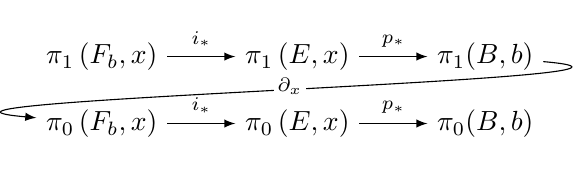
\begin{tikzpicture}[descr/.style={fill=white,inner sep=1.5pt}]
        \matrix (m) [
            matrix of math nodes,
            row sep=1em,
            column sep=2.5em,
            text height=1.5ex, text depth=0.25ex
        ]
        { \pi_1\left(F_b,x\right) & \pi_1\left(E,x\right) & \pi_1(B,b) \\
          \pi_0\left(F_b,x\right) & \pi_0\left(E,x\right) & \pi_0(B,b) \\
        };

        \path[overlay,->, font=\scriptsize,>=latex]
        (m-1-1) edge node[auto] {$i_*$} (m-1-2)
        (m-1-2) edge node[auto] {$p_*$} (m-1-3)
        (m-1-3) edge[out=355,in=175] node[descr,yshift=0.3ex] {$\partial_x$} (m-2-1)
        (m-2-1) edge node[auto] {$i_*$} (m-2-2)
        (m-2-2) edge node[auto] {$p_*$} (m-2-3);
\end{tikzpicture}
\end{center}

as well as the isomorphisms of sets $\partial_x:\frac{\pi_1(B,b)}{p_*\pi_1(E,x)}\cong\pi_0\left(F_b,x\right),i_*:\frac{\pi_0\left(F_b,x\right)}{\pi_1(B,b)}\cong\pi_0(E,x)$

For a covering $p:E\to B$ with $B$ path connected, the exact sequence simplifies to

\begin{center}
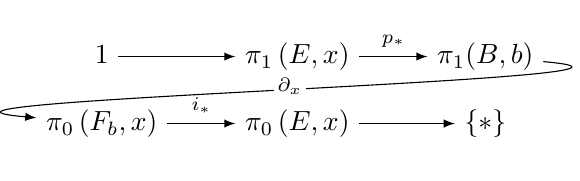
\begin{tikzpicture}[descr/.style={fill=white,inner sep=1.5pt}]
        \matrix (m) [
            matrix of math nodes,
            row sep=1em,
            column sep=2.5em,
            text height=1.5ex, text depth=0.25ex
        ]
        { 1                       & \pi_1\left(E,x\right) & \pi_1(B,b) \\
          \pi_0\left(F_b,x\right) & \pi_0\left(E,x\right) & \{*\}      \\
        };

        \path[overlay,->, font=\scriptsize,>=latex]
        (m-1-1) edge (m-1-2)
        (m-1-2) edge node[auto] {$p_*$} (m-1-3)
        (m-1-3) edge[out=355,in=175] node[descr,yshift=0.3ex] {$\partial_x$} (m-2-1)
        (m-2-1) edge node[auto] {$i_*$} (m-2-2)
        (m-2-2) edge (m-2-3);
\end{tikzpicture}
\end{center}

Furthermore suppose that $p:E\to B$ is a right $G$-principal covering with $E$ path connceted, then we get the exact sequence

\begin{center}
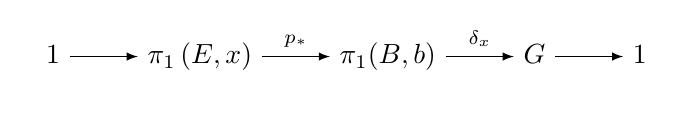
\begin{tikzpicture}[descr/.style={fill=white,inner sep=1.5pt}]
        \matrix (m) [
            matrix of math nodes,
            row sep=1em,
            column sep=2.5em,
            text height=1.5ex, text depth=0.25ex
        ]
        { 1 & \pi_1\left(E,x\right) & \pi_1(B,b) & G & 1 \\
        };

        \path[overlay,->, font=\scriptsize,>=latex]
        (m-1-1) edge (m-1-2)
        (m-1-2) edge node[auto] {$p_*$} (m-1-3)
        (m-1-3) edge node[auto] {$\delta_x$} (m-1-4)
        (m-1-4) edge (m-1-5);
\end{tikzpicture}
\end{center}

and the image of $p_*$ is normal.

\subsection{Coverings}

Outline:
\begin{enumerate}
    \item Construct the inverse $X$ of $T:\TRA_B\to\COV_B$ that exists and is an equivalence of categories for sufficiently nice $B$
    \item Construct the functor $\epsilon_B:\TRA_B\to\pi_b\hyp\SET$ and the inverse $\eta_b$
    \item Hence $A(p):G\hyp\SET\to\COV_B$ is an equivalence of categories iff the total space of $p$ is simply connected
\end{enumerate}

Let $\TRA_B=[\Pi(B),\SET]$, the transport functor in the previous section yields the functor $T:\COV_B\to\TRA_B$.

If $B$ is path connected and $T$ is an equivalence of categories, then $B$ is a \textbf{transport space}.

A set $U\in B$ is \textbf{transport simple} if any paths in $U$ between identical points are homotopic in $B$.

$B$ is \textbf{semi-locally simply connected} if it has an open covering with transport simple sets.

$B$ is \textbf{transport local} if it is path connected, locally path connected and semi-locally simply connected.

\begin{thm*}
    If $B$ is  then $B$ is a transport space
\end{thm*}

\begin{proof}
    We need to construct the inverse of $T$, $X:\TRA_B\to\COV_B$. Let $\Phi:\Pi(B)\to\SET$ be some functor, we will construct a covering $p:X(\Phi)\to B$. As a set $X(\Phi)=\coprod_{b\in B}\Phi(b)$. To get a reasonable topology on it, we consider a covering $\mc U$ of $B$ by transport simple path connected open sets. For every $b\in U\in\mc U$, we define $\phi_{U,b}:U\times\Phi(b)\to p^{-1}(U)$ and by gluing these maps together, we obtain a topology on $X(\Phi)$ and a covering $p$.
    
    Verification of functoriality and inverse are somewhat direct from definition.
\end{proof}

With this, consider the hom functor $\Hom_{\Pi(B)}\left(b,-\right)\in\TRA_B$ and let $p^b:E^b\to B$ be its associated covering. Then $E^b$ is simply connected right $\Hom_{\Pi(B)}\left(b,b\right)$-principal covering.

Suppose that $B$ is path connected, then $\Pi=\Pi(B)$ is a connected groupoid. Let $\Pi(x,y)=\Hom_{\Pi(B)}(x,y)$ and $\pi_b=\Pi(b,b)$

For a functor $F:\Pi\to\SET$, we have the left $\pi_B$-set $F(b)$ giving us the functor $\epsilon_b:\TRA_B\to\pi_b\hyp\SET$.

For a left $\pi_B$-set $A$, we define the functor $\Pi(b,-)\times_{\pi_B}A:\Pi\to\SET$ where $A\times_GB$ is the set $A\times B$ quotiented by $(ag,b)=(a,gb)$. This gives us the functor $\eta_b:\pi_b\hyp\SET\to\TRA_B$, the inverse of $\epsilon_b$.

Finally we have the following categories and functors:

\[\begin{tikzcd}
	G\hyp\SET & \COV_B & \TRA_B & \pi_b\hyp\SET
	\arrow["{A(p)}", from=1-1, to=1-2]
	\arrow["T", curve={height=-6pt}, from=1-2, to=1-3]
	\arrow["X", curve={height=-6pt}, from=1-3, to=1-2]
	\arrow["\simeq"{description}, draw=none, from=1-2, to=1-3]
	\arrow["{\epsilon_b}", curve={height=-6pt}, from=1-3, to=1-4]
	\arrow["{\eta_b}", curve={height=-6pt}, from=1-4, to=1-3]
	\arrow["\simeq"{description}, draw=none, from=1-3, to=1-4]
\end{tikzcd}\]

where $X$ exists if $B$ is transport-local and $\epsilon_B,\eta_B$ require $B$ to be path connected to exist.

Finally we have

\begin{thm*}
    The following are equivalent:
    \begin{itemize}
        \item $B$ is a transport space, i.e. $T$ is an equivalence of categories
        \item $B$ has a universal right $G$-principal covering $p:E\to B$, i.e. $A(p)$ is an equivalence of categories
    \end{itemize}
\end{thm*}

Note that the exact sequences above imply that $E$ is simply connected.

Define the \textbf{orbit category} $\Or(G)$ consisting of homogenous $G$-sets ($\frac GH$ for any subgroup $H$) and $G$-maps. This category is a strict subcategory of $G\hyp\SET$, consisting only the transitive sets.

For a covering $p:E\to B$, we obtain the injective map $p_*:\pi_1(E,x)\to\pi_1(B,p(x))$ and the image is called the \textbf{characteristic subgroup} of $p$ wrt $x$.

Let $p:E\to B$ be a simply connected covering, then the subcategory $A(p)\left(\Or(\pi_b)\right)$ of $\COV_B$ is equivalent to the subcategory consisting of connected coverings. This tells us that the connected coverings of a transport space is determined by subgroups of the fundamental group.

\begin{thm*}
    Let $B$ be a transport space and $p:E\to B$ a covering.
    \begin{itemize}
        \item The action of $\Aut(p)$ on $E$ makes it a left-$\Aut(p)$ principal covering
        \item A simply connected covering is a universal covering
        \item Universal coverings are unique up to isomorphism
        \item The automorphism group of a universal cover is isomorphic to $\pi_1(B,b)$
        \item $E^b$ is simply connected
        \item We have a Galois correspondence between isomorphism classes of connected coverings and subgroups of $\pi_1(B,b)$
    \end{itemize}
\end{thm*}


If $B$ is not a transport space but is path connected and locally path connected, then we have a similar result where coverings by path connected total spaces are isomorphic iff the characteristic subgroups are conjugate in $\pi_1(B,b)$.

Suppose we have coverings $p:E\to B$ and $f:Z\to B$, then a covering $\Phi:Z\to E$ such that \begin{tikzcd}
	Z && E \\
	& B
	\arrow["f"', from=1-1, to=2-2]
	\arrow["p", from=1-3, to=2-2]
	\arrow["\Phi", dashed, from=1-1, to=1-3]
\end{tikzcd} exists iff $f_*\pi_1(Z,z)\subset p_*\pi_1(E,x)$ for some $f(z)=p(x)$.

If $X$ is a topological group with identity $x$ and $p:E\to X$ is a covering with $E$ path connected and locally path connected, then for each $e\in p^{-1}(b)$, there exists a unique group structure on $E$ such that $e$ is the identity and $p$ a homomorphism.



\section{Chapter 4}

\subsection{Mapping cylinders}

For a map $f:X\to Y$ \textbf{mapping cylinder} $Z(f)$ is constructed by the pushout

\[\begin{tikzcd}
	{X+X} & {X+Y} \\
	{X\times I} & {Z(f)} \\
	&& Y
	\arrow["{\left<i_0,i_1\right>}"', from=1-1, to=2-1]
	\arrow["{\id+f}", from=1-1, to=1-2]
	\arrow["{\left<j,J\right>}", dashed, from=1-2, to=2-2]
	\arrow["a"', dashed, from=2-1, to=2-2]
	\arrow["q"{description}, dashed, from=2-2, to=3-3]
	\arrow["f"', curve={height=12pt}, from=2-1, to=3-3]
	\arrow["{\left<f,\id\right>}"{description}, curve={height=-12pt}, from=1-2, to=3-3]
\end{tikzcd}\]

We also have $Jq\cong\id$ as $X\times I\cong X$ and $f=qj$, $j$ a closed immersion and $q$ a homotopy equivalence. We see that $Z$ has nice functorial properties. Suppose we have the homotopy commutative diagram

\[\begin{tikzcd}
	X & Y \\
	{X'} & {Y'} \\
	{X''} & {Y''}
	\arrow["f", from=1-1, to=1-2]
	\arrow["\alpha"', from=1-1, to=2-1]
	\arrow["\beta", from=1-2, to=2-2]
	\arrow["{\alpha'}"', from=2-1, to=3-1]
	\arrow["{f'}"{description}, from=2-1, to=2-2]
	\arrow["{\beta'}", from=2-2, to=3-2]
	\arrow["{f''}"{description}, from=3-1, to=3-2]
\end{tikzcd}\]

and let the homotopy equivalences be $\Phi:f'\alpha\cong\beta f,\Phi':f''\alpha'\cong\beta'f'$

This induces the following homotopy commutative diagram

\[\begin{tikzcd}
	{X+Y} & {Z(f)} \\
	{X'+Y'} & {Z(f')} \\
	{X''+Y''} & {Z(f'')}
	\arrow["{\alpha+\beta}"', from=1-1, to=2-1]
	\arrow["{\alpha'+\beta'}"', from=2-1, to=3-1]
	\arrow[from=1-1, to=1-2]
	\arrow[from=3-1, to=3-2]
	\arrow[from=2-1, to=2-2]
	\arrow["{Z(\alpha,\beta,\Phi)}", from=1-2, to=2-2]
	\arrow["{Z(\alpha',\beta',\Phi'')}", from=2-2, to=3-2]
\end{tikzcd}\]

where each small square commutes in $\TOP$ and the whole diagram commutes in $\hTOP$.

Given maps $f:A\to B$ and $g:A\to C$, we can construct the double mapping cylinder by either of the two pushouts:

\[\begin{tikzcd}
	{A+A} & {B+C} \\
	{A\times I} & {Z(f,g)}
	\arrow["{f+g}", from=1-1, to=1-2]
	\arrow["{\left<i_0,i_1\right>}"', from=1-1, to=2-1]
	\arrow[dashed, from=2-1, to=2-2]
	\arrow["{\left<j_0,j_1\right>}", dashed, from=1-2, to=2-2]
\end{tikzcd}\]
\[\begin{tikzcd}
	A & {Z(f)} \\
	{Z(g)} & {Z(f,g)}
	\arrow["{j^B}", from=1-1, to=1-2]
	\arrow["{j^C}"', from=1-1, to=2-1]
	\arrow[dashed, from=2-1, to=2-2]
	\arrow[dashed, from=1-2, to=2-2]
\end{tikzcd}\]

The functorality of the double mapping cylinder can be seem from the following commutative homotopy diagram:

\[\begin{tikzcd}[column sep=3pt,row sep=4pt]
	&&&&& {A+B} \\
	& A &&& {Z(f)} && {A'+B'} \\
	&& {A'} &&& {Z(f')} && {A''+B''} \\
	&&& {A''} &&& {Z(f'')} \\
	& {Z(g)} &&& {Z(f,g)} \\
	{A+C} && {Z(g')} &&& {Z(f',g')} \\
	& {A'+C'} && {Z(g'')} &&& {Z(f'',g')} \\
	&& {A''+C''}
	\arrow[from=2-2, to=3-3]
	\arrow[from=3-3, to=4-4]
	\arrow[from=2-2, to=2-5]
	\arrow[from=2-2, to=5-2]
	\arrow[dashed, from=5-2, to=5-5]
	\arrow[dashed, from=2-5, to=5-5]
	\arrow[from=1-6, to=2-5]
	\arrow[from=6-1, to=5-2]
	\arrow[dashed, from=4-7, to=7-7]
	\arrow[dashed, from=7-4, to=7-7]
	\arrow[dashed, from=3-6, to=6-6]
	\arrow[dashed, from=6-3, to=6-6]
	\arrow[from=5-5, to=6-6]
	\arrow[from=6-6, to=7-7]
	\arrow[from=7-2, to=6-3]
	\arrow[from=8-3, to=7-4]
	\arrow[from=2-7, to=3-6]
	\arrow[from=3-8, to=4-7]
	\arrow[from=3-3, to=6-3, crossing over]
	\arrow[from=4-4, to=7-4, crossing over]
	\arrow[from=4-4, to=4-7, crossing over]
	\arrow[from=3-3, to=3-6, crossing over]
	\arrow[""{name=0, anchor=center, inner sep=0}, from=5-2, to=6-3]
	\arrow[""{name=1, anchor=center, inner sep=0}, from=6-3, to=7-4]
	\arrow[""{name=2, anchor=center, inner sep=0}, from=2-5, to=3-6]
	\arrow[""{name=3, anchor=center, inner sep=0}, from=3-6, to=4-7]
	\arrow[""{name=4, anchor=center, inner sep=0}, from=1-6, to=2-7]
	\arrow[""{name=5, anchor=center, inner sep=0}, from=2-7, to=3-8]
	\arrow[""{name=6, anchor=center, inner sep=0}, from=6-1, to=7-2]
	\arrow[""{name=7, anchor=center, inner sep=0}, from=7-2, to=8-3]
	\arrow[shorten <=9pt, shorten >=9pt, Rightarrow, from=7, to=1]
	\arrow[shorten <=9pt, shorten >=9pt, Rightarrow, from=4, to=2]
	\arrow[shorten <=9pt, shorten >=9pt, Rightarrow, from=5, to=3]
	\arrow[shorten <=9pt, shorten >=9pt, Rightarrow, from=6, to=0]
\end{tikzcd}\]

Suppose we have the homotopy commutative diagram

\[\begin{tikzcd}
	{X_0} & {X_+} & \\
	{X_-} & X \\
	& & {Z\left(f_-,f_+\right)} \\
	\arrow["{f_+}", from=1-1, to=1-2]
	\arrow["{f_-}"', from=1-1, to=2-1]
	\arrow["{j_+}", from=1-2, to=2-2]
	\arrow["{j_-}"', from=2-1, to=2-2]
	\arrow[curve={height=-12pt}, dashed, from=1-2, to=3-3]
	\arrow[curve={height=12pt}, dashed, from=2-1, to=3-3]
	\arrow["\phi"{description}, dashed, from=3-3, to=2-2]
\end{tikzcd}\]

The square is called a \textbf{homotopy pushout} or \textbf{homotopy cocartesian} if $\phi$ is a homotopy equivalence (i.e. a pushout in the category $\hTOP$)

Let $f_\pm,j_\pm$ be inclusions and $X=X_+\cup X_-$, then the diagram is a pushout in $\TOP$.

Let $N\left(X_-,X_+\right)=X_-\times0\cup X_0\times I\times X_+\times 1$ be a subspace of $X\times I$ and let $p_N:N\left(X_-,X_+\right)\to X$ be the projection map.

The covering $X_\pm$ is \textbf{numerable} if $p_N$ has a section. With this, we have the following condition to determine if the diagram above is a pushout in $\hTOP$:

\begin{thm}
    $Z\left(f_-,f_+\right)\cong X$ if the covering $X_\pm$ is numerable
\end{thm}

Given the projection maps $X\overset f\leftarrow X\times Y\overset g\to Y$, the double mapping cylinder $Z(f,g)=X\star Y$ is known as the \textbf{join} of $X$ and $Y$

\subsection{Suspensions and loops}

Here we work in pointed categories

The \textbf{suspension} functor $\Sigma:\TOP^0\to\TOP^0$ is given by
\begin{itemize}
    \item $\Sigma X=S^1\wedge X=\frac{X\times I}{X\times\partial I\cup\{x\}\times I}$
    \item $S\Sigma_*\left[X,Y\right]^0=\left[\Sigma X,\Sigma Y\right]^0$
\end{itemize}

Note that $\Sigma_*$ is a homomorphism if $X=\Sigma A$ and any pointed homotopy $H_t:X\to Y$ corresponds uniquely to a pointed map $\overline K:\Sigma X\to Y$

The set $\left[\Sigma X,Y\right]^0$ has a natural group structure by composition of homotopies. Furthermore as $\left[\Sigma^nX,Y\right]^0$ has $n$ natural composition laws by composin the homotopies at the the $i$th coordinate and these satisfies the assumptions of Eckmann-Hilton argument, they are equivalent. This also tells us that the higher homotopy groups, $\pi_n(X)=\left[S^n,X\right]^0$, are commutative groups.

We can dualize everything above:

The \textbf{loop} space of $X$ is $\Omega X=F^0\left(S^1,X\right)$. This consists of loops in $X$ with basepoint $x$. This is naturally a topological group with the product of loops. 

There is a natural group structure on $\Hom_{\TOP^0}\left(X,\Omega Y\right)$ given by $[f]+_m[g]=[f][g]$.

As $S^1$ is locally compact, we have the tensor-hom adjuncation

\[\left[\Sigma X,Y\right]^0\cong\left[X,\Omega Y\right]^0\]

and this commutes with the group operation.

In the set $\left[\Sigma X,\Omega Y\right]^0$, by the Eckmann-Hilton argument, the group operations on these two sets coincide and are commutative.

\subsection{Group objects}

Perhaps a nicer way of looking at group/any objects is via Yoneda's lemma, see \cite{Waterhouse-Grp-schemes} for more details:

\begin{thm}[Yoneda]
    For any category $C$, we have a full and faithful functor, the Yoneda embedding $y_C:C\to\left[C^{\op},\SET\right]$, given by $y_C(c)\to\Hom_C\left(-,c\right)$
\end{thm}

An object $g\in C$ is a \textbf{group object} if the functor $y_C(g)$ factors through $\GRP$, i.e. the following diagram commutes where $\GRP\to\SET$ is the forgetful functor

\[\begin{tikzcd}
	& \GRP & \\
	{C^{\op}} && \SET \\
	\arrow[hook, from=1-2, to=2-3]
	\arrow["{y_C(g)}"', from=2-1, to=2-3]
	\arrow["G", dashed, from=2-1, to=1-2]
\end{tikzcd}\]

To give an explicit construction, recall that for a group $G$, we need to have a unit element, an inverse operation and a group operation, given by

\begin{align*}
    e_G&:1\to G\\
    \text{inv}_G&:G\to G^{\op}\\
    \cdot_G&:G\times G\to G
\end{align*}

such that the following diagrams commute to ensure associativity, unit and inverse holds:

\[\begin{tikzcd}
	{G\times G\times G} & {G\times G} && G & {G\times G} && G & {G\times G}\\
	{G\times G} & G && {G\times G} & G && {G\times G} & G
	\arrow["{\cdot_G}"', from=2-1, to=2-2]
	\arrow["{\cdot_G}", from=1-2, to=2-2]
	\arrow["{\cdot_G\times \id_G}"', from=1-1, to=2-1]
	\arrow["{\id_G\times\cdot_G}", from=1-1, to=1-2]
	\arrow[Rightarrow, no head, from=1-4, to=2-5]
	\arrow["{\left(e,\id_G\right)}", from=1-4, to=1-5]
	\arrow["{\cdot_G}", from=1-5, to=2-5]
	\arrow["{\left(\id_G,\text{inv}_G\right)}"', from=1-7, to=2-7]
	\arrow["{\left(\text{inv}_G,\id_G\right)}", from=1-7, to=1-8]
	\arrow["{\cdot_G}", from=1-8, to=2-8]
	\arrow["{\cdot_G}"', from=2-7, to=2-8]
	\arrow["{\left(\id_G,e\right)}"', from=1-4, to=2-4]
	\arrow["{\cdot_G}"', from=2-4, to=2-5]
	\arrow["e"{description}, from=1-7, to=2-8]
\end{tikzcd}\]

where $e:G\to G$ is the composite morphism $G\to 1\overset{e_G}\to G$

The maps can immediately be constructed by Yoneda's lemma, take for instance the product map. If $g$ is a group object with $G:C^{\op}\to\GRP$ as the functor to group and $f:c\to d$ is a morphism in $C$, then the following diagram commutes:

\[\begin{tikzcd}
	{G(c)\times G(c)} & {G(c)} \\
	{G(d)\times G(d)} & {G(d)}
	\arrow["{\cdot_{G(d)}}"', from=2-1, to=2-2]
	\arrow["{\cdot_{G(c)}}", from=1-1, to=1-2]
	\arrow["{G(f)}"', from=2-2, to=1-2]
	\arrow["{G(f)\times G(f)}", from=2-1, to=1-1]
\end{tikzcd}\]

telling us we have a natural transformation $\cdot_G:G\times G\to G$. This gives us the morphism $\cdot_g:g\times g\to g$ by Yoneda's lemma and as the Yoneda embedding is full and faithful, the commutativity of the diagrams above defining a group is immediate.

Similarly one defines cogroups as group objects in the opposite category. With this view, it is immediate that if $c\in C$ is a cogroup, then $\Hom_C(c,-)$ is a functor to $\GRP$.

As examples in $\hTOP^0$, $\Sigma X$ is a cogroup as $\left[\Sigma X,Y\right]^0$ is a group and $\Omega Y$ is a group as $\left[X,\Omega Y\right]^0$ is a group.

\subsection{Fibre sequence}

Again here we work in pointed spaces. A map $f:X\to Y$ induces a map $f^*:[Y,B]^0\to[X,B]^0$. The kernels of $f$ is any element that gets sent to the basepoint of $Y$ and the kernel of $f^*$ is any element that gets sent to a nullhomotopic element. This allows us to define exact sequences of topological spaces.

A sequence of spaces $U\overset f\to V\overset g\to W$ is \textbf{h-coexact} if for all spaces $B$, the sequence
\[[U,B]^0\overset{f^*}\leftarrow[V,B]^0\overset{g^*}\leftarrow[W,B]^0\]
is exact.

The \textbf{cylinder} $XI=\frac{X\times I}{*\times I}$ describes homotopies in $\TOP^0$ (morphisms $XI\to Y$ are homotopies).

The \textbf{cone} $CX=\frac{X\times I}{X\times 0\cup*\times I}=X\wedge I$ describes homotopies starting from constant maps in $\TOP^0$.

Define $C(f)$ as the pushout

\[\begin{tikzcd}
	X & Y \\
	CX & {C(f)}
	\arrow["f", from=1-1, to=1-2]
	\arrow["{i_1}"', from=1-1, to=2-1]
	\arrow["j"', from=2-1, to=2-2]
	\arrow["{f_1}", from=1-2, to=2-2]
\end{tikzcd}\]

and by its universal property, we have the h-coexact sequence $X\overset f\to Y\overset{f_1}\to C(f)$ which can be iterated to create a long h-coexact sequence

\[X\overset f\to Y\overset{f_1}\to C(f)\overset{f_2}\to C\left(f_1\right)\overset{f_3}\to\dots\]

Furthermore we have the commutative diagram

\[\begin{tikzcd}
	X & CX & {Y/i_1X} & {=\Sigma X} \\
	Y & {C(f)} & {C(f)/f_1Y} & {=\Sigma X} \\
	CY & {C\left(f_1\right)} & {C\left(f_1\right)/j_1Y} & {=\Sigma X}
	\arrow["{i_1}", from=1-1, to=1-2]
	\arrow["f"', from=1-1, to=2-1]
	\arrow["{f_1}"{description}, from=2-1, to=2-2]
	\arrow["j", from=1-2, to=2-2]
	\arrow["{i_1}"', from=2-1, to=3-1]
	\arrow["{f_2}", from=2-2, to=3-2]
	\arrow["{j_1}"', from=3-1, to=3-2]
	\arrow["p", from=1-2, to=1-3]
	\arrow["{p(f)}"{description}, from=2-2, to=2-3]
	\arrow["{q(f)}"', from=3-2, to=3-3]
	\arrow[from=1-3, to=2-3]
	\arrow[from=2-3, to=3-3]
\end{tikzcd}\]

Applying this to itself, we obtain

\[\begin{tikzcd}
	X & CX \\
	Y & {C(f)} & {\Sigma X} \\
	CY & {C\left(f_1\right)} \\
	& {C\left(f_2\right)} & {\Sigma Y}
	\arrow["f"', from=1-1, to=2-1]
	\arrow[from=1-1, to=1-2]
	\arrow[from=1-2, to=2-2]
	\arrow[from=2-1, to=3-1]
	\arrow[from=3-1, to=3-2]
	\arrow["{f_3}"', from=3-2, to=4-2]
	\arrow["{q\left(f_1\right)}"', from=4-2, to=4-3]
	\arrow[from=2-2, to=2-3]
	\arrow["{f_2}"', from=2-2, to=3-2]
	\arrow["{f_1}", from=2-1, to=2-2]
	\arrow["{q(f)}"', from=3-2, to=2-3]
	\arrow["{p\left(f_1\right)}", from=3-2, to=4-3]
	\arrow["{\Sigma f\circ\iota}", from=2-3, to=4-3]
\end{tikzcd}\]

where $\iota:(x,t)\to(x,1-t)$ to ensure commtuativity.

As $q(f),q\left(f_1\right)$ are homotopy equivalences and a sequence remains h-coexact if we replace elements with h-equivalent ones, we obtain the h-coexact sequence

\[X\to Y\to C(f)\to\Sigma X\to\Sigma Y\]

And we can apply this sequence to itself iteratively and noting that $\Sigma$ and $C$ commutes to obtain the \textbf{Puppe-sequence} or the \textbf{cofibre sequence} of $f$:

\[X\to Y\to C(f)\to\Sigma X\to\Sigma Y\to\Sigma C(f)\to\Sigma C(f)\to\Sigma^2X\to\Sigma^2Y\dots\]

as $\Sigma f:\Sigma X\to\Sigma Y$

Applying the functor $\left[-,B\right]^0$, we see that from the 4th place onwards these are groups and from the 7th place onwards these are abelian groups.

For any map $f:X\to Y$, let $\mu:C(f)\to\Sigma X\vee C(f)$ be defined as 
\[\mu(x,t)=\begin{cases}\left((x,2t),*\right)&2t\leq 1\\\left(*,(x,2t-1)\right)&2t\geq 1\end{cases}\]
and $\mu(y)=y$. This map is a \textbf{h-coaction} of the h-cogroup $\Sigma X$ on $C(f)$ as we have
\[\left[\Sigma X,B\right]^0\times\left[C(f),B\right]^0\cong\left[\Sigma X\vee C(f),B\right]^0\to\left[C(f),B\right]\]

where the last map is induced by $\mu$. 

With the map $Y\overset{f_1}\to C(f)\overset{p(f)}\to\Sigma X$ and any maps $\alpha_1,\alpha_2:\Sigma X\to B$, this group action satisfies $\left(\alpha_1\right)\left(p(f)^*\alpha_2\right)=p(f)^*\left(\alpha_1\alpha_2\right)$ and $f_1^*$ is an injective map on orbits of this action.

We can dualize everything as always.

A sequence of spaces $U\overset f\to V\overset g\to W$ is \textbf{h-exact} if for all spaces $B$, the sequence
\[[B,U]^0\overset{f^*}\to[B,V]^0\overset{g^*}\to[B,W]^0\]
is exact.

To dualize the cone, we use the exponential object adjuncation $\left[X\wedge I,Y\right]^0\cong\left[X,F^0(Y,I)\right]^0$ and define $FY=F^0(Y,I)$. We then define $F(f)$ as the pullback

\[\begin{tikzcd}
	{F(f)} & FY \\
	X & Y
	\arrow["f"', from=2-1, to=2-2]
	\arrow["{e^1}", from=1-2, to=2-2]
	\arrow["{f^1}"', dashed, from=1-1, to=2-1]
	\arrow["q", dashed, from=1-1, to=1-2]
\end{tikzcd}\]

and by its universal property, we have the h-exact sequence $F(f)\overset{f_1}\to X\overset f\to Y$ which can be iterated to create a long h-exact sequence

\[\dots\overset{f^4}\to F\left(f^2\right)\overset{f^3}\to F\left(f^1\right)\overset{f^2}\to F(f)\overset{f^1}\to X\overset f\to Y\]

We can dualize the diagrams above to obtain

\[\begin{tikzcd}
	Y & FY & {\Omega Y} \\
	X & {F(f)} & {\Omega Y} \\
	FX & {F\left(f^1\right)} & {\Omega Y}
	\arrow["{e^1}"', from=1-2, to=1-1]
	\arrow["f", from=2-1, to=1-1]
	\arrow["{f^1}"{description}, from=2-2, to=2-1]
	\arrow["q"', from=2-2, to=1-2]
	\arrow["i"', from=1-3, to=1-2]
	\arrow["{e^1}", from=3-1, to=2-1]
	\arrow["{f^2}"', from=3-2, to=2-2]
	\arrow["{q^1}", from=3-2, to=3-1]
	\arrow["{i(f)}"{description}, from=2-3, to=2-2]
	\arrow[from=2-3, to=1-3]
	\arrow[from=3-3, to=2-3]
	\arrow["{j(f)}", from=3-3, to=3-2]
\end{tikzcd}\]

where $j(f)$ is a h-equivalence and using this on itself, we obtain

\[\begin{tikzcd}
	Y & FY \\
	X & {F(f)} & {\Omega Y} \\
	FX & {F\left(f^1\right)} \\
	& {F\left(f^2\right)} & {\Omega X}
	\arrow[from=1-2, to=1-1]
	\arrow["f", from=2-1, to=1-1]
	\arrow["{f^1}"', from=2-2, to=2-1]
	\arrow[from=2-2, to=1-2]
	\arrow[from=3-1, to=2-1]
	\arrow["{f^2}", from=3-2, to=2-2]
	\arrow[from=3-2, to=3-1]
	\arrow["{i(f)}"', from=2-3, to=2-2]
	\arrow["{i\left(f^1\right)}"', from=4-3, to=3-2]
	\arrow["{j(f)}", from=2-3, to=3-2]
	\arrow["{f^3}", from=4-2, to=3-2]
	\arrow["{j\left(f^1\right)}", from=4-3, to=4-2]
	\arrow["{\iota\circ\Omega f}"', from=4-3, to=2-3]
\end{tikzcd}\]

and finally we obtain the dual long h-exact sequence

\[\Omega X\to\Omega Y\to F(f)\to X\to Y\]

and repeating this on the map $\Omega f:\Omega X\to\Omega Y$, we obtain the long h-exact sequence

\[\dots\Omega^2X\to\Omega^2Y\to\Omega F(f)\to\Omega X\to\Omega Y\to F(f)\to X\to Y\]

known as the \textbf{fibre seqence} of $f$. Similarly applying the functor $\left[B,-\right]^0$, we see that from the 4th place onwards these are groups and from the 7th place onwards these are abelian groups.

Finally to dualize the group action, again let $f:X\to Y$ be any map. We have the h-action $m:\Omega Y\times F(f)\to F(f)$ defined as

\[m\left(\left[f(t),\left(x,g(t)\right)\right]\right)=\begin{cases}\left(x,f(2t)\right)&2t\leq1\\\left(x,g(2t-1)\right)&2t\geq1\end{cases}\]

This map induces the map

\[\left[B,\Omega Y\right]^0\times\left[B,F(f)\right]^0\cong\left[B,\Omega Y\times F(f)\right]^0\to\left[B,F(f)\right]^0\]

Furthermore with the maps $\Omega Y\overset{i(f)}\to F(f)\overset{f^1}\to X$ and any maps $\alpha_1,\alpha_2:B\to\Omega Y$, this group action satisfies $\left(i(f)_*\alpha_1\right)\left(\alpha_2\right)=i(f)_*\left(\alpha_1\alpha_2\right)$ and $f^1_*$ is an injective map on the orbits of the action.

\section{Chapter 5}

\begin{thebibliography}{99}
    \bibitem[May]{May-concise} May, J. P. (1999). A concise course in algebraic topology. University of Chicago press.
    \bibitem[Wat]{Waterhouse-Grp-schemes} Waterhouse, W. C. (2012). Introduction to affine group schemes (Vol. 66). Springer Science \& Business Media.
\end{thebibliography}

\end{document}
